\subsection{Daten zwischen Widgets teilen}
Aufgrund der Art und Weise wie \textit{Flutter} entworfen wurde,
können Daten zwischen Widgets nur von oben nach unten
beziehungsweise vom Eltern- zum Kind-Widget übergeben werden.
In der unten stehenden Abbildung ist das Eingabeformular der App zu sehen.
Dieses besteht wie bereits erwähnt aus verschiedenen Widgets.
Jede \textit{"Zeile"} ist ein Widget und enthält wiederum Widgets
wie Formularfelder, \textit{Checkboxen} oder \textit{Chips}.
Auf der Ebene des Formulars selbst, aber in der Abbildung nicht zu sehen,
ist der Button zum senden der Daten. Würde das Formular ausschließlich
aus Formularfeldern bestehen, wäre dies auch kein größeres Problem.
In diesem Fall könnte man auf sämtliche Formularfelder direkt zugreifen.
Jedoch besteht das Formular auch aus solchen Widgets die Listen
repräsentieren und keine klassischen Formularfelder sind.
Diese beiden Bereiche sind in der Abbildung cyanfarben umrandet.
Zum einen kann eine Pizza mehrere Toppings und zum anderen
gleichzeitig verschiedene Typen annehmen.

\begin{figure}[H]
    \centering
    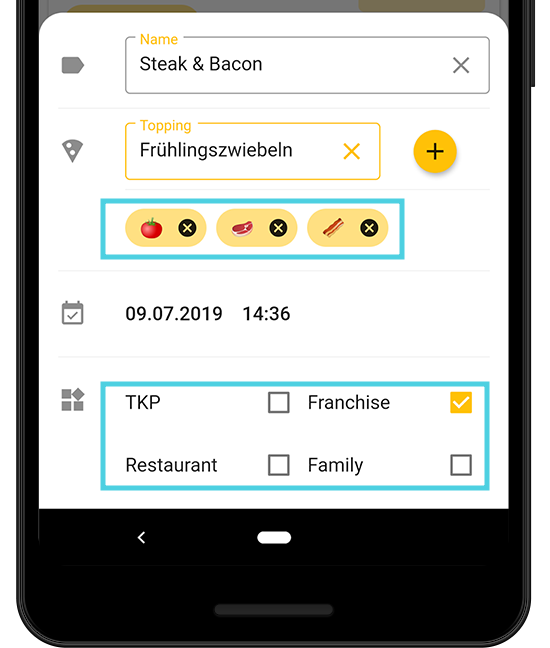
\includegraphics[width=0.4\columnwidth]{pixel-3_mockup-4--shared-data}
    \caption{App: Formular mit Shared-Data}
\end{figure}

Da diese Listen eine Ebene tiefer als der Button zum Absenden der Daten liegen,
kann es keinen direkten Zugriff geben.
In \textit{Flutter} gibt es grundsätzlich zwei Arten wie Daten übergeben werden können:

\begin{enumerate}
    \itemsep-0.4em
    \item Daten über den Konstruktor des Widgets hinzufügen
    \item \textit{Flutter}'s \textit{BuildContext}
\end{enumerate}

\newpage

Jedem Widget steht die Klasse \textit{BuildContext} zur Verfügung.
Diese erlaubt es einem Widget, mit Hilfe der folgenden Methoden
Daten von jedem Vorfahren anzufordern.

\begin{itemize}
    \itemsep-0.4em
    \item \textit{inheritFromWidgetOfExactType(Type)}
    \item \textit{ancestorStateOfType(TypeMatcher)}
    \item \textit{ancestorWidgetOfExactType(Type)}
\end{itemize}

Besonders abfrageintensiven Operationen empfiehlt
sich \textit{inheritFromWidgetOfExactType(Type)}.
Diese Methoden gehören zur Basis-Klasse \textit{InheritedWidget}.
Solche \textit{Inherited}-Widgets lösen einen Rebuild im Konsumenten
aus wenn deren State geändert wurde.
Um das Handling mit diesen Methoden zu vereinfachen,
nutze ich das Paket \textit{provider}. Welches vor allem
\textit{Syntax Sugar} für \textit{InheritedWidget} bietet.
Um Daten einfach zwischen Widgets teilen zu können,
empfiehlt es sich, sogenannte Daten-Klassen zur
Haltung sowie Manipulation dieser zu vereinfachen.
Dies kann nach folgendem Muster gelöst werden:

\begin{figure}[H]
    \centering
    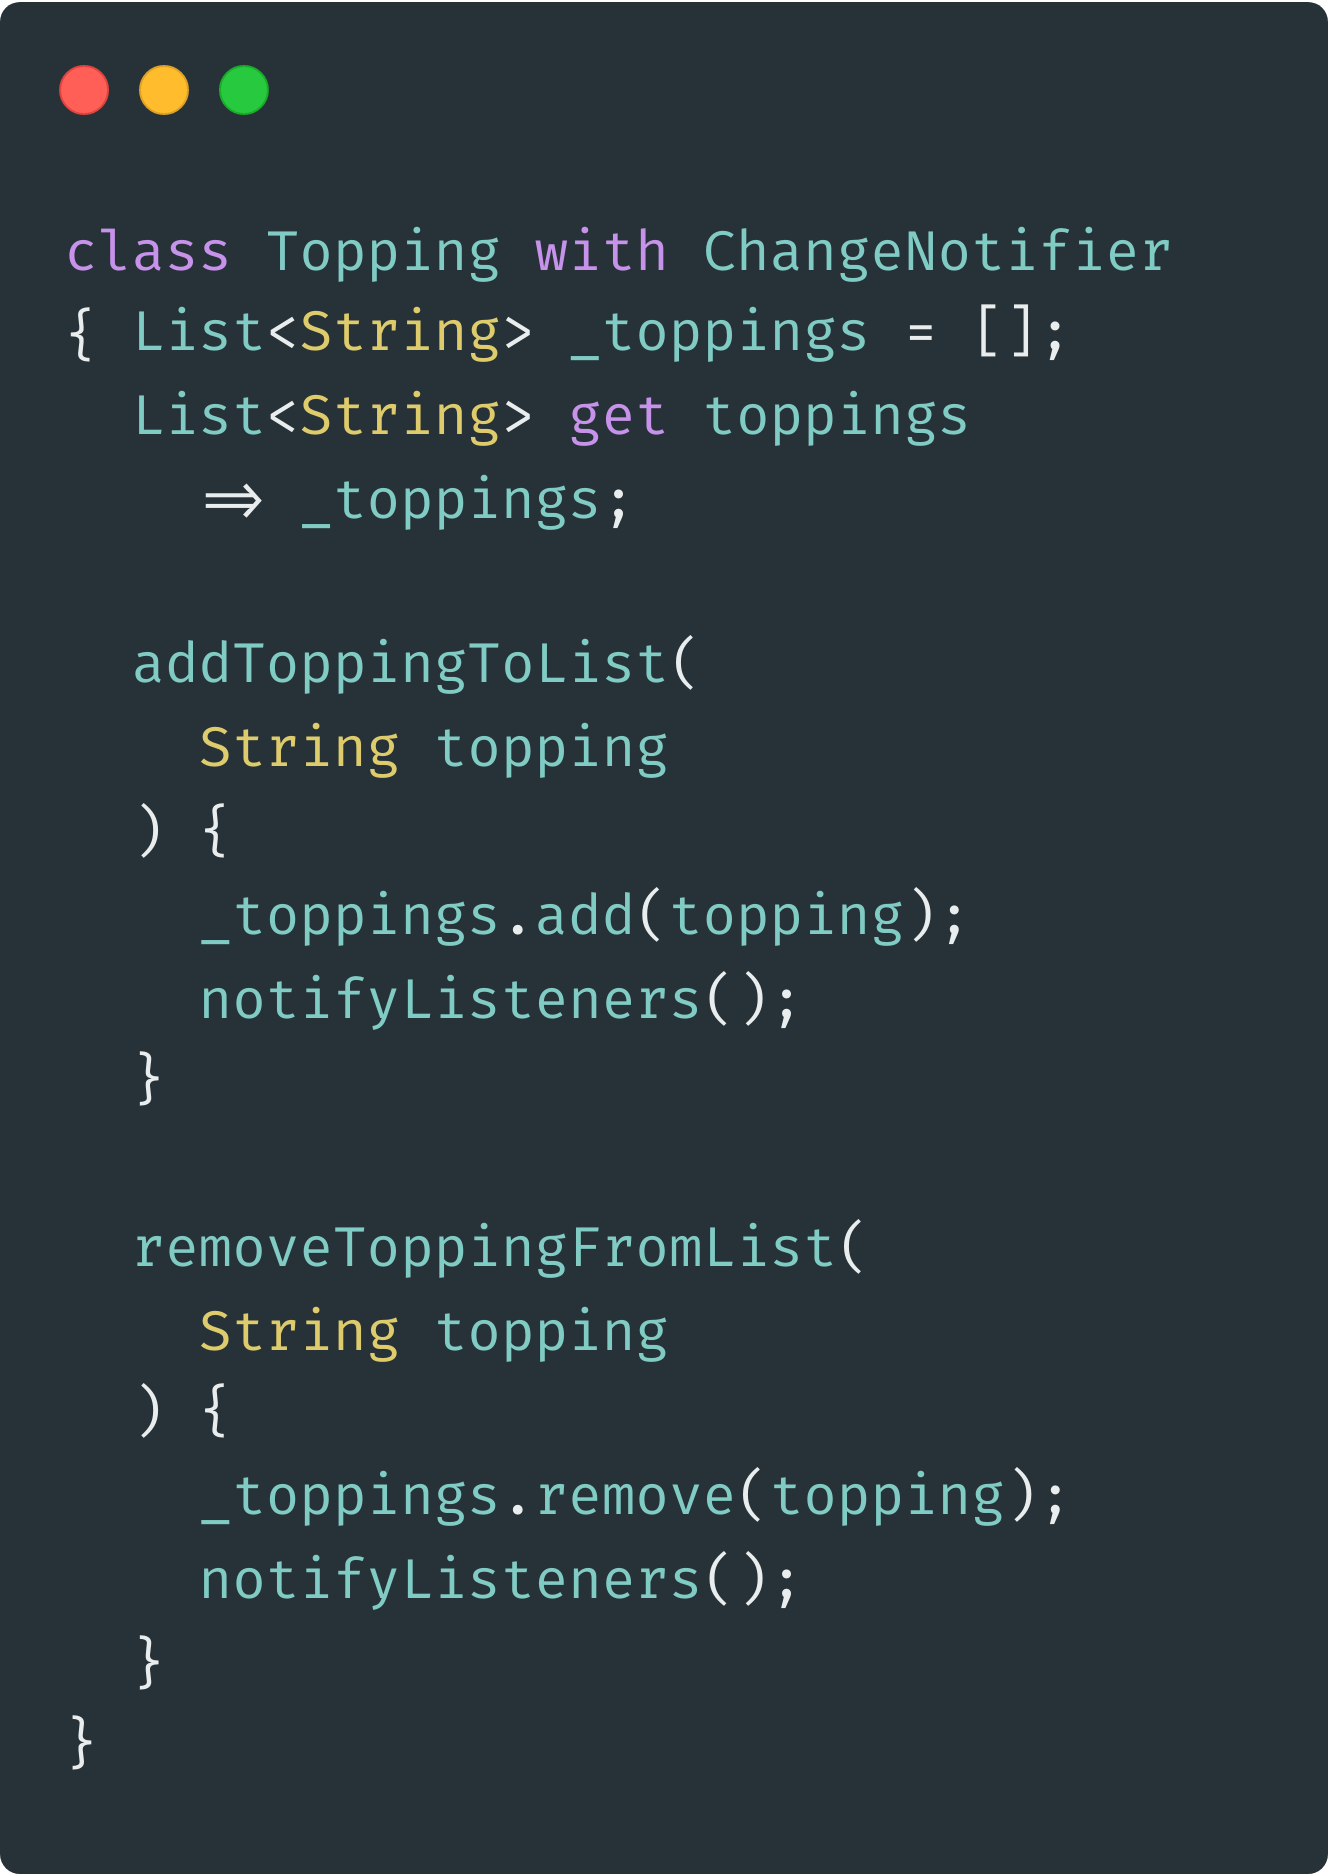
\includegraphics[width=0.4\columnwidth]{topping_change-notifier}
    \caption{Dart: ChangeNotifier}
\end{figure}

Über das sogenannte \textit{Mixin "ChangeNotifier"} lassen
sich Eigenschaften und Methoden dieser Klasse auf die eigene Daten-Klasse
übertragen. Die in den Methoden \textit{addToppingToList} \& \textit{removeToppingToList}
aufgerufene Methode \textit{notifyListeners} informiert das Formular immer dann darüber,
dass Änderungen an den Listen stattgefunden haben.
Somit ändert sich der State der Widgets an sich sowie des Formulars, welches wiederum
einen Rebuild auslöst.
Um diese Daten-Klassen dann im Formular nutzen zu können,
müssen die Provider eine Ebene höher, in diesem Fall in der \textit{main.dart}
wie folgt eingebunden werden:

\begin{figure}[H]
    \centering
    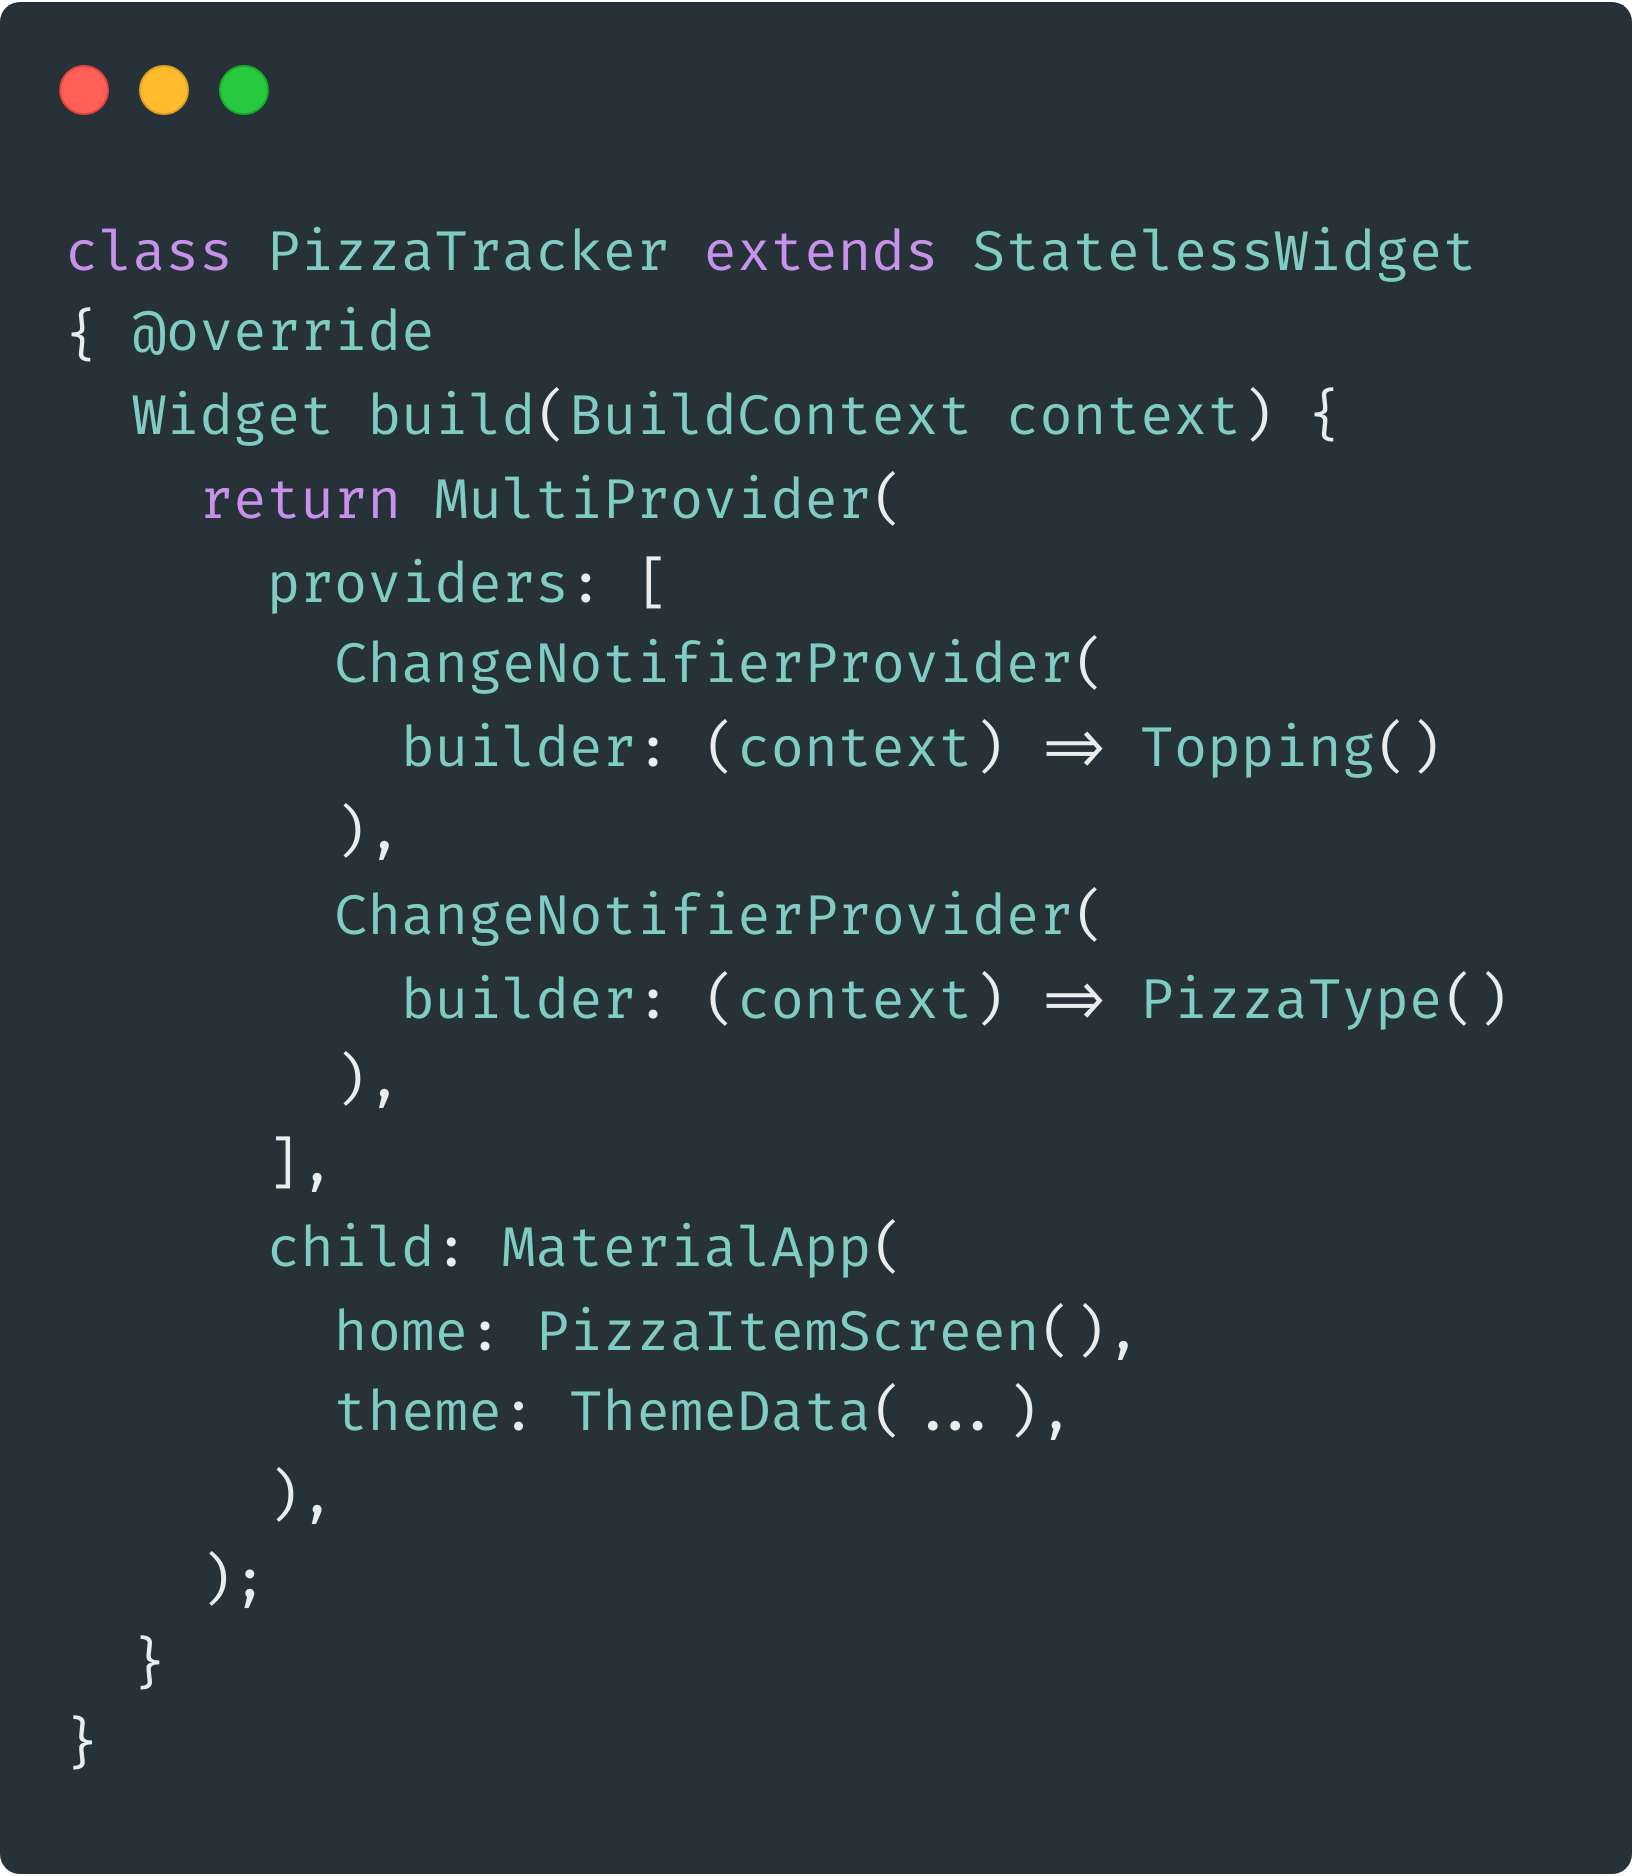
\includegraphics[width=0.4\columnwidth]{multi_provider}
    \caption{Dart: MultiProvider}
\end{figure}

\newpage
